%!TEX root = ../VorlageBA.tex
\chapter{Data modeling techniques and information system }
  
\section{ Data modeling techniques}
A model is an abstraction and reflection of the real world. Modeling gives us the capacity to visualize what we can not yet figure it out. The essential point of the modeling is to ensure that all information objects required by the business are precisely and completely represented.\\

E/R model is the traditional way of data modeling. The focus of E/R model is to capture the relationship between different elements. The dimensional modeling comparatively new technique than E/R model. Both models have some similarities and some differences. In the following sections, discussing basics of dimensional modeling and E/R modeling techniques.



\subsection{Dimensional Modeling}

\begin{quotation}
	\textit{\enquote{A methodology for logically modeling data to maximize analytic query performance and ease of use.}}\footnote{(Kimball, M., p.534)} 
\end{quotation} 
The dimensional modeling is very popular in data warehousing because its query performance for large queries is better compare to E/R model. It consist typically two types of tables, fact and dimensional table. This type of dimensional model is also known as star schema. \\

The fact table and dimensional table have different characteristics.\newline
The fact table normally contains numerical values. For example, quantity, price or profit etc. Fact table contains related dimensional tables keys called foreign keys in the fact table.Compare to dimensional table the fact table has less column but large numbers of rows. The numeric value of the fact table use to create different business answer. For instance, how many cars sold in last month or total last month revenue.\newline

The dimensional table contains the detail information about facts.For example, car type, engine type, car color, parts supplier. Those information are useful for analysis. Normally the dimension table contains large number of column because it is containing all related descriptive data. \\
There are three basic types of dimensional model exist, they are
\begin{itemize}
\item Star model
\item Snowflake model
\item Multi-star model or Galaxy schema
\end{itemize}
Star model have one fact table and multiple dimensional table.\\
In the snowflake model, dimensions are containing the other dimensional data.\\
In the multi-star fact model consist of  multiple fact table and multiple dimension. The common dimension for each fact table is called as conformed dimension. \footnote{(Ballard, D., Dimensional Modeling, p.52-58)} \\\\
\begin{figure}[!ht] 
	\centering
		%[natürliche Breite in Pixeln, natürliche Höhe in Pixeln, Abhängigkeit von der Textbreite]
		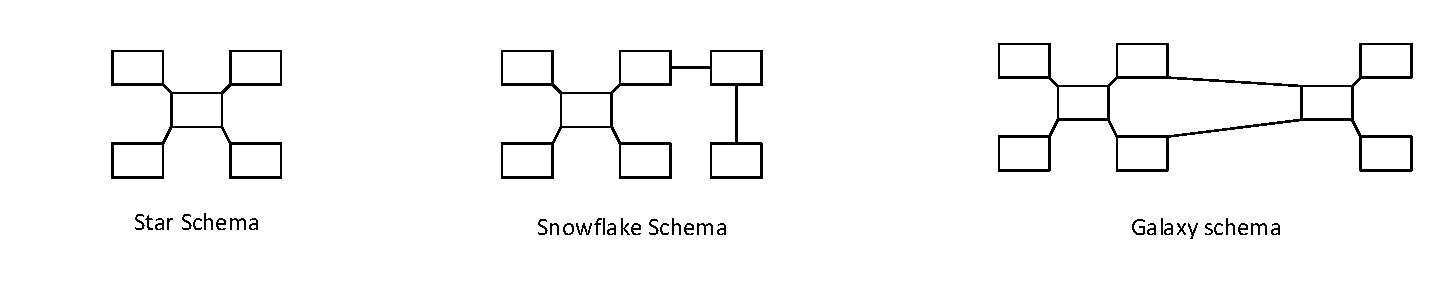
\includegraphics[width=pt, height=134pt, width=1.0\textwidth]{images/todm.pdf}
	\caption[Types of dimensional model]{Types of dimensional model\footnotemark}
	\label{fig:TODM }
\end{figure}
\footnotetext{(Ballard, D., Dimensional Modeling, p.56)}

According to the Kimball dimensional modeling approach, data should be dimensionally organized. There are four steps for dimensional design process.
\begin{enumerate}
\item Select the business process 
\item Declare the grain
\item Identify the dimensions
\item Identify the facts
\end{enumerate}

\label{sec:section}

The first step is to select the business process means the operational activities which are performing by the organization. The performance metrics translate into the fact in the fact table. Picking the business process is vital because it characterizers the particular target design, permit the grain, measurements and dimensions.\\

The second step is to declare the grain. This is an important part for dimensional design process. Declare the grain means what exactly the single fact table row represents. It gives the response to the inquiry, "How do you describe a single row in a fact table?". Grain should be declare before defining the dimensional tables. \\

In the third step is to identify the dimension to the fact table. After declare the grain it is easy to find out the dimensions. Dimensions provides the "who, what, where, when, and how" context surrounding the business process. It contains the descriptive attributes of the fact table and can be use for filtering and grouping the the facts.  \\

The last step of the dimensional design process is to identify the facts. Declaring the grain for the fact table will helps to identify the facts. It gives the answer, " What is the process measuring?". This results helps to business user to analyze the process and present the status of the business. Fact tables normally contains the measurement values and the foreign keys of the dimensional table which are related to the fact table. A single fact table row has a one-to-one relationship to a measurement event as describe by the fact table grain. \footnote{(Kimball and Ross, 2013, p.70-72)}

\begin{figure}[!ht]
	\centering
		%[natürliche Breite in Pixeln, natürliche Höhe in Pixeln, Abhängigkeit von der Textbreite]
		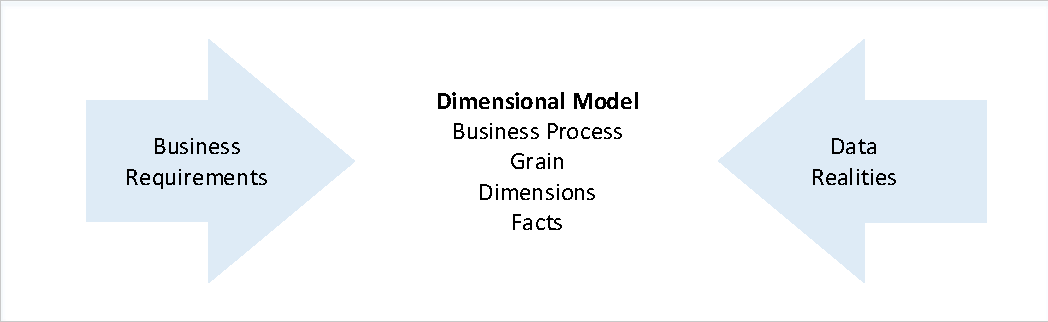
\includegraphics[width=pt, height=156pt, width=1.0\textwidth]{images/fsddp.pdf}
	\caption[Key input to the four-step dimensional design process.]{Key input to the four-step dimensional design process\footnotemark} 
	\label{fig:showcase}

\end{figure}
\footnotetext{(Kimball and Ross, 2013, p.72)}
\subsection{E/R modeling}
E/R modeling  is a data modeling techniques in which store the data  in highly  
normalize form inside the relational database table. Big tables split into smaller tables and each table contain a primary key and independent attributes which can be identified by primary key. This types of data structure known as third normal form (3NF). The main goal of this type of  data structure is reduce the redundancy of data. The E/R model mainly concentrates on three things, entity, attribute and relationship.

According to Inmon data modeling approach there are there levels:
\begin{enumerate}
\item High level modeling (called the entity relationship diagram,or ERD)
\item Midlevel modeling (called data item set, or DIS)
\item Low-level modeling (called physical model) 
\end{enumerate}

Figure 2.3 shows high level of the entity relationship model. The entities represent by oval, the connection between two entity with single direction arrow represent 1:N relationship and arrow with both direction represents M:N relationship. The entities in the E/R level represent the  highest level of abstraction. In the ERD level it is necessary to define the which entities are belongs to the scope of model and which are not.
\begin{figure}[!ht]
	\centering
		%[natürliche Breite in Pixeln, natürliche Höhe in Pixeln, Abhängigkeit von der Textbreite]
		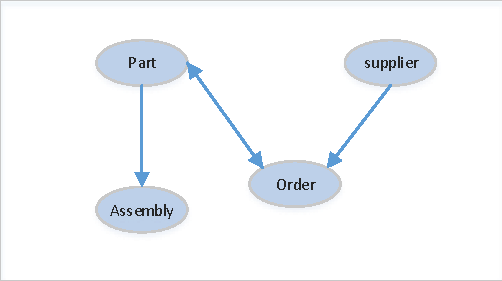
\includegraphics[width=226pt, height=132pt, width=1.0\textwidth]{images/inmon1.pdf}
	\caption[Entity and Relationship]{Entity and Relationship\footnotemark} 
	\label{fig:Inmon}

\end{figure}
\footnotetext{(Inmon, 2005, p.82)}

In the midlevel, data modle derive from the high level data model. Each entity in the high level data model called as major subject area. In this midlevel, create midlevel model for each subject area. There are four basic activity found in this level. They are :
\begin{itemize}
\item A primary grouping of data
\item Secondary grouping of data
\item A connector
\item Type of data

\end{itemize}

Primary grouping contain attributes, keys and it exists only once for each major subject area. In the secondary grouping attributes can exist multiple times. A connector use to make relationship between groups. Left side grouping data called super type and right side grouping data called as subtype.\\

The physical level extend the midlevel by including the keys and physical characteristics  of the model. At this level the series of table are build which also called as relational table.\footnote{(Inmon, 2005, p.82-88)} \newpage

\section{ Information System}
Information System plays an important role for an organization in various ways. It is supporting in business operation, managerial decision and many more. In an organization there are different managerial levels and different types of information are needed.  In the following section, discussing about the view point of the information system, derivation of information requirements and key points of the information quality management. 
\subsection{View point of Information System}
\begin{figure}[!ht]
	\centering
		%[natürliche Breite in Pixeln, natürliche Höhe in Pixeln, Abhängigkeit von der Textbreite]
		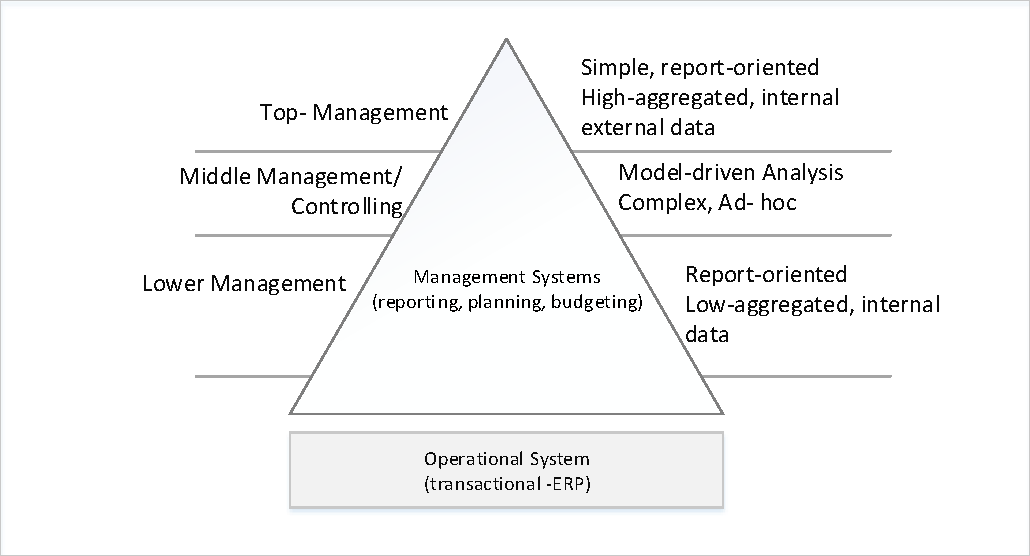
\includegraphics[width=530pt, height=280pt, width=1.0\textwidth]{images/info1.pdf}
	\caption[Traditional view point of information system]{Traditional view point of information system\footnotemark} 
	\label{fig:Inmon}

\end{figure}
\footnotetext{(Westenberger, 2014, p.12)}

From Figure 2.4 seen the traditional view point of information system. Top management mainly responsible for strategic decision making and establish objectives for the whole organization in long term basis. Top management require less data compare to any other management in the organization but those data are highly aggregated with the combination of internal and external data. Those information also known as key figure of the organization. For example, total revenue, total sales etc.\newline

Middle level management focus on tactical information of the organization. They are responsible for different analysis of the business process for assigning assets and setting up controls to execute the best process for the organization. This level of manager require more data compare to top management but less aggregation, mainly they focus on ad-hoc reports.\newline

Low level managers require  detail report of a specific part of the operational activities. The operational information  relates to current and historical performance and is based mainly on internal data.

\subsection{Derivation of Information Requirements}

In an organization there are different strategic objectives. Those objectives can not directly support by information system. At first, those strategic objectives and goals need to classified into different  actions. From the different actions it is possible to define the required information which will support to the strategic objectives. For example, the organizational goal would be more customer should be focus  on the company or increase quality of the product. Then action would be invest on production or take a survey after product delivery. The required information would be the complain rate, customer classification or contacts.\footnote{Westengerber,2014, P.27-30 }  

\begin{figure}[!ht]
	\centering
		%[natürliche Breite in Pixeln, natürliche Höhe in Pixeln, Abhängigkeit von der Textbreite]
		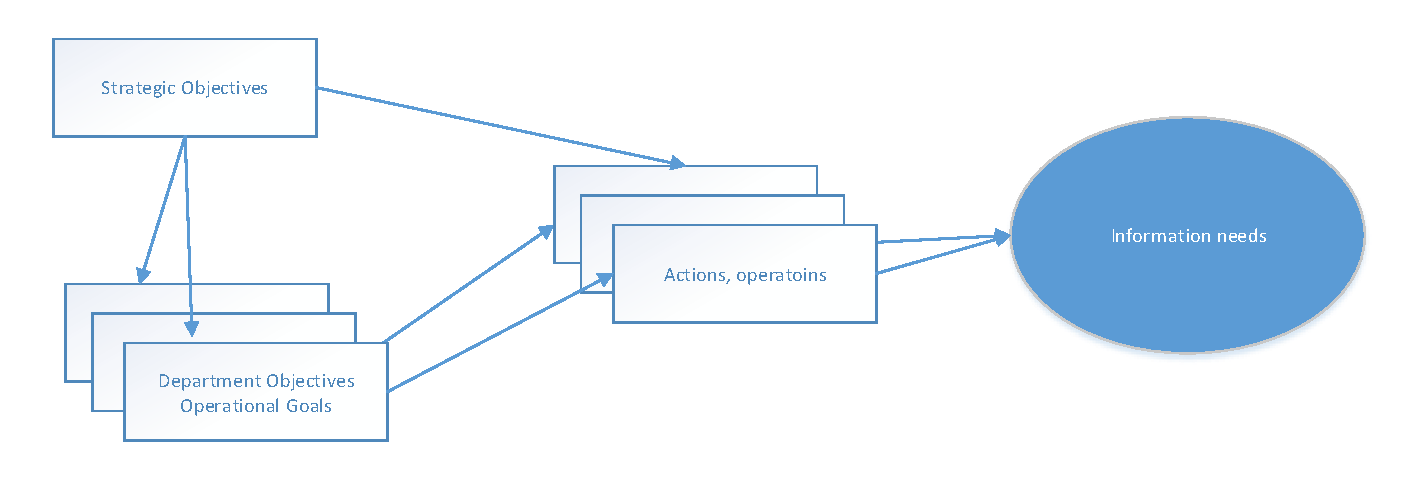
\includegraphics[width=845pt, height=258pt, width=1.0\textwidth]{images/info2.pdf}
	\caption[Derivation of Information Requirements]{Derivation of Information Requirements\footnotemark} 
	\label{fig:Info2}

\end{figure}
\footnotetext{(Westenberger, 2014, p.27)}
\subsubsection{Key Performance Indicator}
Key Performance Indicators, or KPIs, are a tool for organizations use to gauge exactly how viably they are accomplishing their objectives. Utilizing KPIs is a route for organizations to measure their business goals so they can consistently investigate their execution and figure out where they are fruitful and where they have to make strides. The KPIs a business takes after will rely on its specific industry, and keeping in mind that a few measurements will be critical over an association, every office will likewise likely track measurements particular to its own objectives.
KPIs can be utilized inside an organization or division to track its objectives and decide how best to calibrate its center practices to accomplish the best outcomes. \\

Examples of Key Performance Indicators 
\begin{itemize}
\item Actual cost of work done - In the project management 
\item Return on Asset/ Return on Equity - IN Financial management
\item Number of reworks/ Failure/ Car painted - In automotive industry
\end{itemize}

\subsection{Information Quality}
Information quality in an important part of the information system. Most of the decision making process depends on current information.Wrong information can affects the quality of decision making. A good management information system have to ensure the quality of the information. Information quality in a multi attribute concept. There are different characteristics that can define the information quality. The key characteristics of the quality information are:
\begin{itemize}
\item Accuracy
\item Reliability
\item Relevance
\item Completeness
\item Timeliness
\item Cost/Benefit
\item Uniqueness
\end{itemize}

The data stores in the database it should represent the exact data what was captured. The higher precision of the data shows the better information quality. Besides the data accuracy, the data reliability is a key characteristic of the data quality.The  understanding of the reliability comes from the quality of the sources, the approach embraced to gain and process the data and the channel of the delivery.It is also important to get complete data which will represent the reality. As well as timeliness security also important. \\

To maintain the data quality some guidelines can be follow. The guidelines are mentioning below.

\subsubsection{Data stewardship}
Understand the roles and responsibility in data ownership, acquisition, quality assurance, storage and distribution then establish individual functional area which will count own performance. 
\subsubsection{Data element development and specification}
Develop and maintain data, system and reporting mechanisms for sound data management and quality for end user service. 
\subsubsection{Data and quality standards}
Develop internal standards where it is applicable and harmonize the standards across the various system.
\subsubsection{Data management and data quality tools}
Develop tools such as data dictionary, business rules, data flow documentation, process flow and mapping
\subsubsection{Measurement}
Develop performance metrics to measure data quality issues and presents the results for each data source
\subsubsection{Privacy}
Train users about the data privacy issues, policies and compliance with the privacy regulations.\footnote{Prevosto and Marotta, 2005, https://www.iqint.org/publication2011/doc2/prevosto-2005-04.pdf }













